%\documentclass{beamer}
\documentclass[handout]{beamer} % to skip transitions

%%\input{Qcircuit.tex}
\usepackage[braket]{qcircuit}
\usepackage{mathtools}
\usepackage{amsmath}
\usepackage{hyperref}
\usepackage{enumerate}
\usepackage{xmpmulti}

%%%%%%%%%%%%%%%%%%%%%%%%%%%%%%%%%%%%%%%%%%%%%%%%%%%%%%%%%%%%%%%%%%%%%%%%%%%%%%%%

\usetheme{default}
\setbeamertemplate{navigation symbols}{} 

%%%%%%%%%%%%%%%%%%%%%%%%%%%%%%%%%%%%%%%%%%%%%%%%%%%%%%%%%%%%%%%%%%%%%%%%%%%%%%%%

\newcommand{\C}{{\mathbb{C}}}
\newcommand{\F}{{\mathbb{F}}}
\newcommand{\R}{{\mathbb{R}}}
\newcommand{\Z}{{\mathbb{Z}}}

\newcommand{\cH}{\mathcal{H}}

\DeclareMathOperator{\tr}{tr}
\DeclareMathOperator{\spn}{span}
\DeclareMathOperator{\poly}{poly}
\DeclareMathOperator{\lcm}{lcm}
\renewcommand{\d}{{\mathsf{d}}}
\newcommand{\ii}{{\mathsf{i}}}

\newcommand{\norm}[1]{\|{#1}\|}
\newcommand{\Norm}[1]{\left\|{#1}\right\|}
\newcommand{\floor}[1]{{\lfloor{#1}\rfloor}}
\newcommand{\ceil}[1]{{\lceil{#1}\rceil}}
\newcommand{\nint}[1]{{\lfloor{#1}\rceil}}
\newcommand{\amp}[2]{a_{{#1}|{#2}}}

\newcommand{\nicefrac}[2]{\frac{#1}{#2}}
\newcommand{\smfrac}[2]{{\textstyle{\frac{#1}{#2}}}}

\renewcommand{\>}{\rangle}
\newcommand{\<}{\langle}
\newcommand{\ot}{\otimes}

\def\bas#1\eas{\begin{align*}#1\end{align*}}

\theoremstyle{definition}
\newtheorem{prob}{Problem}
\newtheorem{question}{Question}

\newcommand{\lab}[1]{{}} %%\large\color{beamer@blendedblue} #1.} }
\newcommand{\claim}[1][]{\lab{Claim{#1}}}

\newcommand{\overdef}[2]{\begin{tabular}{@{}c@{}} #1 \\[-1.5ex] \color{teal}\footnotesize #2 \end{tabular}}

\newcommand{\overdefloose}[2]{\begin{tabular}{@{}c@{}} #1 \\[-1ex] \color{teal}\footnotesize #2 \end{tabular}}

%%%%%%%%%%%%%%%%%%%%%%%%%%%%%%%%%%%%%%%%%%%%%%%%%%%%%%%%%%%%%%%%%%%%%%%%%%%%%%%%

\title{Brief Introduction to Quantum Algorithms}

\author{Pawel Wocjan\inst{1}}
\institute{
\inst{1} 
IBM Quantum}

\date{}

%%%%%%%%%%%%%%%%%%%%%%%%%%%%%%%%%%%%%%%%%%%%%%%%%%%%%%%%%%%%%%%%%%%%%%%%%%%%%%%%

\begin{document}

\begin{frame}[plain]

\begin{center}

\bigskip
\bigskip

{\usebeamerfont{title}\usebeamercolor[fg]{title}\inserttitle}

\bigskip
\bigskip

\begin{tabular}{c@{\hspace{5ex}}c}
  Pawe{\l} Wocjan \\ 
  \footnotesize Quantum Algorithms Team, IBM Quantum \\ \\
  \footnotesize Physics Department, University of Tokyo \\
  \footnotesize November 2025
\end{tabular}

\end{center}
\end{frame}

%%%%%%%%%%%%%%%%%%%%%%%%%%%%%%%%%%%%%%%%%%%%%%%%%%%%%%%%%%%%%%%%%%%%%%%%%%%%%%%

\begin{frame}{Visit to the University of Tokyo}

I am honored to visit the Department of Physics at the University of Tokyo.
\bigskip

I am especially grateful to \textbf{Professor Mio Murao} for this opportunity.
\bigskip

If you have questions about quantum computing, I’d be delighted to chat during my stay (until November 21st). 

\bigskip
Feel free to talk to me when I’m at the university or contact me via email: \texttt{Pawel.Wocjan@ibm.com}.
\end{frame}


%%%%%%%%%%%%%%%%%%%%%%%%%%%%%%%%%%%%%%%%%%%%%%%%%%%%%%%%%%%%%%%%%%%%%%%%%%%%%%%

\begin{frame}{Context and Focus}

\medskip
With steady progress in quantum hardware, error correction, and fault tolerance,

\bigskip
\textbf{the search for new quantum algorithms for large-scale fault-tolerant quantum computers has become more critical than ever.}

\end{frame}

%%%%%%%%%%%%%%%%%%%%%%%%%%%%%%%%%%%%%%%%%%%%%%%%%%%%%%%%%%%%%%%%%%%%%%%%%%%%%%%

\begin{frame}{Challenges in Design and Analysis of Quantum Algorithms}

\textbf{Sweet Spot:}
Find problems with:
\medskip
\begin{itemize}
    \item Practical relevance
    \medskip
    \item Classical hardness
    \medskip
    \item Quantum efficiency
\end{itemize}

\bigskip
\textbf{Provable quantum advantage:}
Rigorously prove separation between classical and quantum algorithms.

\bigskip
\textbf{Heuristic quantum advantage:}
Test heuristics on large fault-tolerant quantum computers.

\end{frame}

%%%%%%%%%%%%%%%%%%%%%%%%%%%%%%%%%%%%%%%%%%%%%%%%%%%%%%%%%%%%%%%%%%%%%%%%%%%%%%%

\begin{frame}{Some Quantum Subroutines and Algorithms}
\begin{itemize}
    \item Quantum phase estimation \& Quantum Fourier transform
    \medskip
    \item Block encodings, quantum signal processing
    \medskip
    \item Simulation of quantum systems
    \begin{itemize}
        \item Hamiltonian time evolutions
        \item Lindbladian time evolutions
        \item Preparing thermal states (Gibbs sampling)
        \item Preparing ground states
    \end{itemize}
    \medskip
    \item Amplitude amplification and estimation
    \begin{itemize}
        \item Grover's algorithm
        \item Quantum Chebyshev inequality
    \end{itemize}
    \medskip
    \item Quantum walk-based algorithms
\end{itemize}
\end{frame}

%%%%%%%%%%%%%%%%%%%%%%%%%%%%%%%%%%%%%%%%%%%%%%%%%%%%%%%%%%%%%%%%%%%%%%%%%%%%%%%%

\begin{frame}{Some Quantum Subroutines and Algorithms}
\begin{itemize}
    \item Quantum algorithms for
    \begin{itemize}
        \item Linear equations 
        \item Semidefinite programming
        \item Differential equations
    \end{itemize}
    \medskip
    \item Quantum algorithms for the hidden subgroup problem 
    \begin{itemize}
        \item Shor's algorithms for integer factorization \& computing DLOG
        \item Algorithms for computing unit \& class groups of number fields
    \end{itemize}
    \medskip
    \item Quantum algorithms for optimization
    \begin{itemize}
        \item Adiabatic algorithm
        \item Decoded quantum interferometry
    \end{itemize}
    \medskip
    \item Quantum algorithms for problems in topology
    \begin{itemize}
        \item Data analysis
        \item Khovanov homology, Jones and HOMFLYPT polynomials
    \end{itemize}
\end{itemize}
\end{frame}

%%%%%%%%%%%%%%%%%%%%%%%%%%%%%%%%%%%%%%%%%%%%%%%%%%%%%%%%%%%%%%%%%%%%%%%%%%%%%%%%

\begin{frame}{Quantum Circuit Model}

\hspace{1.5cm}
\Qcircuit @C=0.7em @R=0.7em {
\lstick{\ket{1}} & \gate{U_{1\,}}     & \multigate{1}{U_3} & \qw                & \multigate{1}{U_6} & \meter & \rstick{0} \\
\lstick{\ket{1}} & \multigate{1}{U_2} & \ghost{U_3}        & \gate{U_5}         & \ghost{U_6}        & \meter & \rstick{1} \\
\lstick{\ket{0}} & \ghost{U_2}        & \qw                & \multigate{1}{U_6} & \qw                & \meter & \rstick{0} \\
\lstick{\ket{1}} & \multigate{1}{U_3} & \gate{U_4}         & \ghost{U_5}        & \multigate{1}{U_7} & \meter & \rstick{1} \\
\lstick{\ket{0}} & \ghost{U_3}        & \qw                & \qw                & \ghost{U_7}        & \meter & \rstick{1}
}

\bigskip

\bigskip
\textbf{Quantum circuits:} Foundational model for fault-tolerant quantum computing.

\bigskip
\textbf{Qiskit:} Open-source framework for designing, simulating, and running quantum circuits.

\medskip
\url{https://www.ibm.com/quantum/qiskit}

\end{frame}

%%%%%%%%%%%%%%%%%%%%%%%%%%%%%%%%%%%%%%%%%%%%%%%%%%%%%%%%%%%%%%%

%% Quantum Phase Estimation

%%%%%%%%%%%%%%%%%%%%%%%%%%%%%%%%%%%%%%%%%%%%%%%%%%%%%%%%%%%%%%%

\begin{frame}{Quantum Phase Estimation}

Given: A unitary $U$ and eigenvector $|\psi\>$ with unknown eigenphase $\varphi\in[0,1)$ where 

\[
   U|\psi\> = e^{2 \pi i \varphi}|\psi\>
\]

\bigskip
Task: Output an estimate $\hat{\varphi}$ such that
\[
   \Pr\Big(|\hat{\varphi} - \varphi| \le \frac{1}{2^n}\Big) \ge \frac{3}{4}
\]
Deviation $|\hat{\varphi} - \varphi|$ is computed modulo $1$.
\end{frame}


%%%%%%%%%%%%%%%%%%%%%%%%%%%%%%%%%%%%%%%%%%%%%%%%%%%%%%%%%%%%%%%

%% Phase Kick Back

%%%%%%%%%%%%%%%%%%%%%%%%%%%%%%%%%%%%%%%%%%%%%%%%%%%%%%%%%%%%%%%

\begin{frame}{Phase Kick Back: Derivation}

\hspace{4cm}
\Qcircuit @C=1em @R=0.7em {
\lstick{|+\>}    & \ctrl{1} & \qw  \\
\lstick{|\psi\>} & \gate{U} & \qw 
}

\bigskip
\begin{eqnarray*}
\frac{|0\> + |1\>}{\sqrt{2}} \otimes |\psi\>  \pause
&  = &
\frac{|0\>}{\sqrt{2}} \otimes |\psi\> + \frac{|1\>}{\sqrt{2}} \otimes |\psi\> \\ \pause
& \mapsto &
\frac{|0\>}{\sqrt{2}} \otimes |\psi\> + \frac{|1\>}{\sqrt{2}} \otimes U |\psi\> \\ \pause
& = &
\frac{|0\>}{\sqrt{2}} \otimes |\psi\> + \frac{|1\>}{\sqrt{2}} \otimes e^{2\pi i\varphi} |\psi\> \\ \pause
& = &
\frac{|0\>}{\sqrt{2}} \otimes |\psi\> + \frac{e^{2\pi i\varphi} |1\>}{\sqrt{2}} \otimes |\psi\> \\ \pause
& = &
\frac{|0\> + e^{2\pi i\varphi} |1\>}{\sqrt{2}} \otimes |\psi\> 
\end{eqnarray*}

\end{frame}

%%%%%%%%%%%%%%%%%%%%%%%%%%%%%%%%%%%%%%%%%%%%%%%%%%%%%%%%%%%%%%%

%% Phase Kick Back

%%%%%%%%%%%%%%%%%%%%%%%%%%%%%%%%%%%%%%%%%%%%%%%%%%%%%%%%%%%%%%%

\begin{frame}{Phase Kick Back: Summary}

\hspace{4cm}
\Qcircuit @C=1em @R=0.7em {
\lstick{|+\>}    & \ctrl{1} & \qw  \\
\lstick{|\psi\>} & \gate{U} & \qw
}
\bigskip
\[
\frac{|0\> + |1\>}{\sqrt{2}} \otimes |\psi\>  \pause
\mapsto
\frac{|0\> + e^{2\pi i\varphi} |1\>}{\sqrt{2}} \otimes |\psi\>
\]

\bigskip
The eigenstate $|\psi\>$ in the {\color{blue} target} register remains {\color{blue} unchanged}.

\bigskip
$\Rightarrow$ Focus on the control register.

\bigskip
The state $|0\>+|1\>$ of the {\color{red} control} qubit changes to $|0\>+e^{2\pi i \varphi}|1\>$ via phase kick back.
\end{frame}

%%%%%%%%%%%%%%%%%%%%%%%%%%%%%%%%%%%%%%%%%%%%%%%%%%%%%%%%%%%%%%%

%% Phase Kick Back

%%%%%%%%%%%%%%%%%%%%%%%%%%%%%%%%%%%%%%%%%%%%%%%%%%%%%%%%%%%%%%%

\begin{frame}{Hadamard Test + Phase Kick Back}

The Hadamard transformation $H$ is
\begin{align*}
    H 
    &= 
    \frac{1}{\sqrt{2}}
    \left(
    \begin{array}{rr}
         1 &  1 \\
         1 & -1
    \end{array}
    \right)
\end{align*}

The Hadamard test circuit is

\medskip
\hspace{4cm}
\Qcircuit @C=1em @R=0.7em {
\lstick{|0\>}    & \gate{H}    & \ctrl{1} & \gate{H} & \meter \\
\lstick{|\psi\>} & {/}\qw      & \gate{U} & \qw      & \qw
}

\medskip
The second Hadamard gate transforms the state as follows:
\begin{eqnarray*}
&& 
\frac{|0\> + e^{2\pi i\varphi} |1\>}{\sqrt{2}} \\ \pause
& \mapsto &
\frac{1}{2}\, \big( (|0\> + |1\>) + e^{2\pi i\varphi} ( |0\> - |1\> ) \big) \\ \pause
& = &
\frac{1}{2}\, \big( ( 1 + e^{2\pi i\varphi}) |0\> + ( 1 - e^{2\pi i\varphi}) |1\> ) \big)  := |\varphi\> 
\end{eqnarray*}

\end{frame}

%%%%%%%%%%%%%%%%%%%%%%%%%%%%%%%%%%%%%%%%%%%%%%%%%%%%%%%%%%%%%%%

%% Phase Kick Back

%%%%%%%%%%%%%%%%%%%%%%%%%%%%%%%%%%%%%%%%%%%%%%%%%%%%%%%%%%%%%%%

\begin{frame}{Hadamard Test + Phase Kick Back}

\begin{align*}
\Pr(0) 
&=  
\left\| |0\>\<0| \, |\varphi\> \right\|^2 \\
&= 
\left| \frac{1}{2} \, (1 + e^{2\pi i \varphi}) \right|^2 \\
%&=
%\frac{1}{4} \, \left|e^{\pi i\varphi} + e^{-\pi i\varphi}) \right|^2 \\
%&=
%\frac{1}{4} \, \left| 2 \cos(\pi\varphi)\right|^2 \\ 
&=
%\cos^2(\pi\varphi) = 
\frac{1}{2} \, \left(1 +\cos(2\pi\varphi)\right)
\end{align*}

\hspace{2.5cm}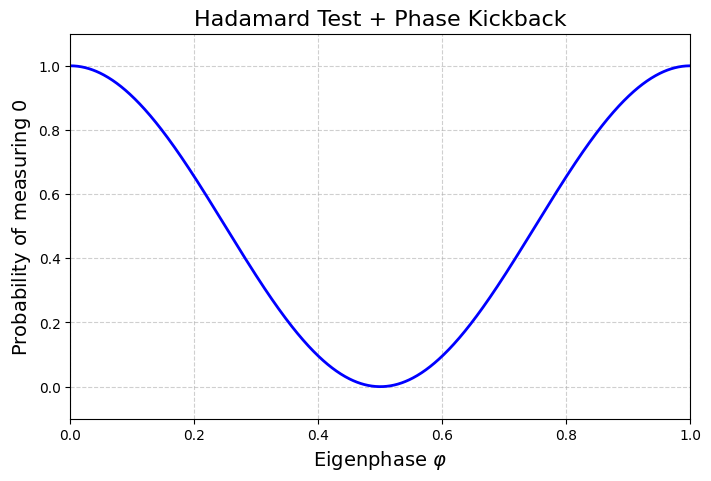
\includegraphics[scale=0.35]{hadamard_test.png}

\end{frame}

%%%%%%%%%%%%%%%%%%%%%%%%%%%%%%%%%%%%%%%%%%%%%%%%%%%%%%%%%%%%%%%%%%%%%%%%%%%%%%%%%%%%%%%%%%%%%%%%%%%%%%%%%%%%

%% Phase kick back 

%%%%%%%%%%%%%%%%%%%%%%%%%%%%%%%%%%%%%%%%%%%%%%%%%%%%%%%%%%%%%%%%%%%%%%%%%%%%%%%%%%%%%%%%%%%%%%%%%%%%%%%%%%%%
\begin{frame}{Phase Kick Back Using Powers of $U$}

	For arbitrary $k$, we obtain
	
	\bigskip
	
	\bigskip
	\hspace{1cm}
	\Qcircuit @C=1.0em @R=1.0em {  
		\lstick{|0\>}    & \qw  &\gate{H}  &  \ctrl{1}       &  \qw  &  \qw &  \qw &  \rstick{\frac{1}{\sqrt{2}}({|0\> + e^{2\pi i 2^k\varphi}|1\>})}\\
	 	\lstick{|\psi\>} & \qw  &{/}\qw    &  \gate{U^{2^k}} &  \qw  &  \qw &  \qw &  \rstick{|\psi\>}
	}			 	
	
	\bigskip
	
	since
	\begin{eqnarray*}
		U^{2^k}|\psi\>=e^{2\pi i 2^k \varphi}|\psi\>
	\end{eqnarray*}

\end{frame}

%%%%%%%%%%%%%%%%%%%%%%%%%%%%%%%%%%%%%%%%%%%%%%%%%%%%%%%%%%%%%%%%%%%%%%%%%%%%

%% Phase estimation

%%%%%%%%%%%%%%%%%%%%%%%%%%%%%%%%%%%%%%%%%%%%%%%%%%%%%%%%%%%%%%%%%%%%%%%%%%%%

\begin{frame}{Phase Kick Back Part of Phase Estimation}

\hspace{1cm}
\Qcircuit @C=1.0em @R=0.7em {
\lstick{|0\>}    & \qw & \gate{H} & \qw      & \qw      & \qw &        & & \qw & \ctrl{4} & \qw & \qw & \rstick{\frac{|0\> + e^{2\pi i 2^{n-1}\varphi}|1\>}{\sqrt{2}}} \\
\lstick{|0\>}    & \qw & \gate{H} & \qw      & \ctrl{3} & \qw &        & & \qw & \qw      & \qw & \qw & \rstick{\frac{|0\> + e^{2\pi i 2^{n-2}\varphi}|1\>}{\sqrt{2}}} \\
                 &     & \raisebox{0.5em}{\vdots}   &          &          &     & \cdots & &     &          &     &     & \rstick{\raisebox{0.5em}{\vdots}} \\
\lstick{|0\>}    & \qw & \gate{H} & \ctrl{1} & \qw      & \qw &        & & \qw & \qw      & \qw & \qw & \rstick{\frac{|0\> + e^{2 \pi i 2^0\varphi}|1\>}{\sqrt{2}}} \\
%
\lstick{|\psi\>} & \qw & {/} \qw  & \gate{U^{2^0}} & \gate{U^{2^1}} & \qw & & & \qw & \gate{U^{2^{n-1}}} & \qw & \qw & \rstick{|\psi\>}
}

\bigskip

\bigskip
We set
\[
|\varphi\> := 
\frac{|0\> + e^{2 \pi i 2^{n-1} \varphi}|1\>}{\sqrt{2}} \!\otimes\!
\frac{|0\> + e^{2 \pi i 2^{n-2} \varphi}|1\>}{\sqrt{2}} \!\otimes\!\cdots\!\otimes
\frac{|0\> + e^{2 \pi i 2^0 \varphi}    |1\>}{\sqrt{2}} 
\]

\end{frame}

%%%%%%%%%%%%%%%%%%%%%%%%%%%%%%%%%%%%%%%%%%%%%%%%%%%%%%%%%%%%%%%%%%%%%%%%%%%

%% Binary fractions

%%%%%%%%%%%%%%%%%%%%%%%%%%%%%%%%%%%%%%%%%%%%%%%%%%%%%%%%%%%%%%%%%%%%%%%%%%%

\begin{frame}{Binary Fractions}

Assume that the eigenphase $\varphi$ is an exact $n$-bit binary fraction, i.e.,
\[
\varphi=0.x_1 x_2 \ldots x_n = \sum_{i=1}^n \frac{x_i}{2^i}
\]

For $k\in\{0,\ldots,n-1\}$, we have
\begin{eqnarray*}
2^k\, \varphi 
& = &
x_1 x_2\ldots x_k . x_{k+1} \ldots x_n \\
& & \\
e^{2\pi i 2^k \varphi} 
&=&
e^{2\pi i (x_1x_2\ldots x_k . x_{k+1}\ldots x_n)}\\
&=&
e^{2\pi i (x_1x_2\ldots x_k + 0. x_{k+1}\ldots x_n)} \\
&=&
e^{2\pi i (x_1x_2\ldots x_k)} \cdot e^{2\pi i (0. x_{k+1}\ldots x_n)} \\
&=& 
e^{2\pi i (0. x_{k+1}\ldots x_n)}
\end{eqnarray*}

\end{frame}

%%%%%%%%%%%%%%%%%%%%%%%%%%%%%%%%%%%%%%%%%%%%%%%%%%%%%%%%%%%%%%%%%%%%%%%%%%%%

%% Phase estimation

%%%%%%%%%%%%%%%%%%%%%%%%%%%%%%%%%%%%%%%%%%%%%%%%%%%%%%%%%%%%%%%%%%%%%%%%%%%%

\begin{frame}{Phase Kick Back Part of Phase Estimation: Summary}

\Qcircuit @C=1.0em @R=0.7em {
\lstick{|0\>}&\qw& \gate{H} & \qw      & \qw      & \qw &        & & \qw & \ctrl{4} & \qw & \qw & \rstick{\frac{|0\> + e^{2\pi i 0.x_n}|1\>}{\sqrt{2}}}\\
\lstick{|0\>}&\qw& \gate{H} & \qw      & \ctrl{3} & \qw &        & & \qw & \qw      & \qw & \qw & \rstick{\frac{|0\> + e^{2\pi i 0.x_{n-1} x_n}|1\>}{\sqrt{2}}}\\
             &   & \raisebox{0.5em}{\vdots}   &          &          &     & \cdots & &     &          &     &     & \rstick{\raisebox{0.5em}{\vdots}} \\
\lstick{|0\>}&\qw& \gate{H} & \ctrl{1} & \qw      & \qw &        & & \qw & \qw      & \qw & \qw & \rstick{\frac{|0\> + e^{2 \pi i 0.x_1 \ldots x_{n-1} x_n}|1\>}{\sqrt{2}}}\\
%
\lstick{|\psi\>} & \qw & {/} \qw  & \gate{U^{2^0}} & \gate{U^{2^1}} & \qw & & & \qw & \gate{U^{2^{n-1}}} & \qw & \qw & \rstick{|\psi\>}
}

\end{frame}

%%%%%%%%%%%%%%%%%%%%%%%%%%%%%%%%%%%%%%%%%%%%%%%%%%%%%%%%%%%%%%%%%%%%%%%%%%%%

%% Quantum Fourier transform

%%%%%%%%%%%%%%%%%%%%%%%%%%%%%%%%%%%%%%%%%%%%%%%%%%%%%%%%%%%%%%%%%%%%%%%%%%%%

\begin{frame}{Quantum Fourier Transform}

The QFT $F$ is defined by

\begin{align*}
&
F \big( |x_n\> \otimes |x_{n-1}\> \otimes \cdots \otimes |x_1\> \big) \\ 
& \\
&=
\frac{|0\> + e^{2 \pi i 0.x_n}|1\>}{\sqrt{2}} \!\otimes\!
\frac{|0\> + e^{2 \pi i 0.x_{n-1} x_n}|1\>}{\sqrt{2}} \!\otimes\!\cdots\!\otimes
\frac{|0\> + e^{2 \pi i 0.x_1x_2\ldots x_n}|1\>}{\sqrt{2}} 
\end{align*}

\bigskip
$\Longrightarrow$ We can use inverse QFT $F^\dagger$ to obtain the bits of the eigenphase.

\end{frame}

%%%%%%%%%%%%%%%%%%%%%%%%%%%%%%%%%%%%%%%%%%%%%%%%%%%%%%%%%%%%%%%%%%%%%%%%%%%%

%% Quantum circuit for phase estimation

%%%%%%%%%%%%%%%%%%%%%%%%%%%%%%%%%%%%%%%%%%%%%%%%%%%%%%%%%%%%%%%%%%%%%%%%%%%%

\begin{frame}{Quantum Circuit for Phase Estimation}

\Qcircuit @C=1.0em @R=0.7em {
\lstick{|0\>}& \qw & \gate{H}                 & \qw      & \qw      & \qw &        &        & \qw & \ctrl{4} & \qw & \multigate{3}{F^\dagger} & \qw & \rstick{|x_n\>}\\
\lstick{|0\>}& \qw & \gate{H}                 & \qw      & \ctrl{3} & \qw &        &        & \qw & \qw      & \qw & \ghost{F^\dagger}        & \qw & \rstick{|x_{n-1}\>}\\
             &     & \raisebox{0.5em}{\vdots} &          &          &     & \cdots &        &     &          &     &         &     & \\
\lstick{|0\>}& \qw & \gate{H}                 & \ctrl{1} & \qw      & \qw &        &        & \qw & \qw      & \qw & \ghost{F^\dagger}        & \qw & \rstick{|x_1\>}\\
%
\lstick{|\psi\>} & \qw & {/} \qw  & \gate{U^{2^0}} & \gate{U^{2^1}} & \qw & & & \qw & \gate{U^{2^{n-1}}} & \qw & \qw & \qw & \rstick{|\psi\>}
}

\bigskip

\bigskip
Let us now derive the quantum circuit for $F^\dagger$.

\end{frame}

%%%%%%%%%%%%%%%%%%%%%%%%%%%%%%%%%%%%%%%%%%%%%%%%%%%%%%%%%%%%%%%%%%%%%%%%%%%

\begin{frame}{Inverse QFT for $3$ bits}

\hspace{2.0cm}
\Qcircuit @C=.4em @R=1.0em {  
\lstick{\frac{|0\> + e^{2\pi i 0.x_3}|1\>}{\sqrt{2}}}       &\qw &\gate{H} & \qw & \qw & \qw & \qw & \ctrl{1}        & \qw & \qw      & \qw & \qw & \qw & \ctrl{2}        & \qw             & \qw & \qw & \qw & \qw & \rstick{|x_3\>} \\ 
\lstick{\frac{|0\> + e^{2\pi i 0.x_2x_3}|1\>}{\sqrt{2}}}    &\qw &\qw      & \qw & \qw & \qw & \qw & \gate{R_2^\dagger} & \qw & \gate{H} & \qw & \qw & \qw & \qw             & \ctrl{1}        & \qw &\qw      &\qw & \qw & \rstick{|x_2\>} \\ 
\lstick{\frac{|0\> + e^{2\pi i 0.x_1x_2x_3}|1\>}{\sqrt{2}}} &\qw &\qw      & \qw & \qw & \qw & \qw & \qw             & \qw & \qw      & \qw & \qw & \qw & \gate{R_3^\dagger} & \gate{R_2^\dagger} & \qw &\gate{H} &\qw & \qw & \rstick{|x_1\>}  
	        \gategroup{1}{3}{1}{3}{1.3em}{--}
	        \gategroup{1}{8}{2}{10}{1.3em}{--}
	        \gategroup{1}{14}{3}{17}{1.3em}{--}
}	

\bigskip
The phase shift $R_k$ is defined by
\[
R_k :=
\left[ 
\begin{array}{cc}
 1 & 0  \\
 0 & e^{2\pi i/2^k}  \\
 \end{array} 
\right]
\]	 
\end{frame}

%%%%%%%%%%%%%%%%%%%%%%%%%%%%%%%%%%%%%%%%%%%%%%%%%%%%%%%%%%%%%%%%%%%%%%%%%%%%

%% least significant bit -- top qubit

%%%%%%%%%%%%%%%%%%%%%%%%%%%%%%%%%%%%%%%%%%%%%%%%%%%%%%%%%%%%%%%%%%%%%%%%%%%%

\begin{frame}{Least Significant Bit -- Top Qubit}

\hspace{3cm}
\Qcircuit @C=1.0em @R=1.0em {  
	\lstick{\frac{|0\>+e^{2\pi i 0.x_3}|1\>}{\sqrt{2}}} &\qw &\gate{H} & \qw & \qw
	\gategroup{1}{3}{1}{3}{1.2em}{--}
}			 	

\bigskip
\begin{eqnarray*}
	&                 & \frac{|0\> + e^{2\pi i 0.x_3}|1\>}{\sqrt{2}} \pause = \frac{|0\> + (-1)^{x_3} |1\>}{\sqrt{2}} \\ \pause
	& \xrightarrow{H} & |x_3\> 
\end{eqnarray*}

\end{frame}

%%%%%%%%%%%%%%%%%%%%%%%%%%%%%%%%%%%%%%%%%%%%%%%%%%%%%%%%%%%%%%%%%%%%%%%%%%%%%

%% second bit -- middle qubit

%%%%%%%%%%%%%%%%%%%%%%%%%%%%%%%%%%%%%%%%%%%%%%%%%%%%%%%%%%%%%%%%%%%%%%%%%%%%%

\begin{frame}{Second Bit -- Middle Qubit}

\hspace{3cm}
\Qcircuit @C=1.0em @R=1.0em {
	\lstick{|x_3\>}                                           & \qw & \ctrl{1}            & \qw      & \qw & \qw \\
	\lstick{\frac{|0\> + e^{2\pi i 0.x_2 x_3}|1\>}{\sqrt{2}}} & \qw & \gate{R_2^\dagger}  & \gate{H} & \qw & \qw 
	\gategroup{1}{3}{2}{4}{1.5em}{--}
}
			              
\bigskip        
\begin{eqnarray*}
		&                                  & |x_3\> \otimes \frac{|0\> + e^{2\pi i 0.x_2 x_3}|1\>}{\sqrt{2}} \\ \pause
		& \xrightarrow{ctrl\, R_2^\dagger} & |x_3\> \otimes \frac{|0\> + e^{2\pi i 0.x_2 0}  |1\>}{\sqrt{2}} \\ \pause
    & \xrightarrow{I \otimes H}				 & |x_3\> \otimes |x_2\> 
\end{eqnarray*} 

\end{frame}

%%%%%%%%%%%%%%%%%%%%%%%%%%%%%%%%%%%%%%%%%%%%%%%%%%%%%%%%%%%%%%%%%%%%%%%%%%%%%

%% most significant bit -- bottom qubit

%%%%%%%%%%%%%%%%%%%%%%%%%%%%%%%%%%%%%%%%%%%%%%%%%%%%%%%%%%%%%%%%%%%%%%%%%%%%%

\begin{frame}{Most Significant Bit -- Bottom Qubit}

\hspace{3cm}
\Qcircuit @C=1.0em @R=1.0em {
	\lstick{|x_3\>}                                        & \qw & \ctrl{2}           & \qw                &\qw      & \qw & \qw \\
	\lstick{|x_2\>}                                        & \qw & \qw                & \ctrl{1}           &\qw      & \qw & \qw \\
	\lstick{\frac{|0\> + e^{0.x_1 x_2 x_3}|1\>}{\sqrt{2}}} & \qw & \gate{R_3^\dagger} & \gate{R_2^\dagger} &\gate{H} & \qw & \qw
	\gategroup{1}{3}{3}{5}{1.5em}{--}
}

\bigskip
\begin{eqnarray*}
			& & 																	  |x_3\> \otimes |x_2\> \otimes \frac{|0\> + e^{2\pi i 0.x_1 x_2 x_3}|1\>}{\sqrt{2}}  \\ \pause
			& \xrightarrow{ctrl\, R_3^\dagger}    & |x_3\> \otimes |x_2\> \otimes \frac{|0\> + e^{2\pi i 0.x_1 x_2 0  }|1\>}{\sqrt{2}}  \\ \pause
  		& \xrightarrow{ctrl\, R_2^\dagger}    & |x_3\> \otimes |x_2\> \otimes \frac{|0\> + e^{2\pi i 0.x_1 0   0  }|1\>}{\sqrt{2}}  \\ \pause
  		& \xrightarrow{I \otimes I \otimes H} & |x_3\> \otimes |x_2\> \otimes |x_1\> 
\end{eqnarray*} 
\end{frame}

%%%%%%%%%%%%%%%%%%%%%%%%%%%%%%%%%%%%%%%%%%%%%%%%%%%%%%%%%%%%%%%%%%%%%%%%%%%%

%% Summary of phase estimation circuit

%%%%%%%%%%%%%%%%%%%%%%%%%%%%%%%%%%%%%%%%%%%%%%%%%%%%%%%%%%%%%%%%%%%%%%%%%%%%

\begin{frame}{Summary of Phase Estimation Circuit}


  Phase kick back using the controlled $U^{2^k}$ gate prepares the state

  \medskip
  		\[
  				\frac{|0\> + e^{2 \pi i 0.x_{k+1} x_{k+2}\ldots x_n} |1\>}{\sqrt{2}}
  		\] \pause
  
  Phase shifts controlled by the previously determined bits $x_{k+2},\ldots, x_n$ transforms it to

  \medskip
  	  \[
  	  		\frac{|0\> + e^{2 \pi i 0.x_{k+1} 0 \ldots 0  } |1\>}{\sqrt{2}} = \frac{|0\> + (-1)^{x_{k+1}}|1\>}{\sqrt{2}}
  	  \] \pause
  
  The Hadamard gate transforms it to
  	\[
  			|x_{k+1}\>
  	\] \pause
  	
\end{frame}

%%%%%%%%%%%%%%%%%%%%%%%%%%%%%%%%%%%%%%%%%%%%%%%%%%%%%%%%%%%%%%%%%%%%%%%%%%%%

%% Special case

%%%%%%%%%%%%%%%%%%%%%%%%%%%%%%%%%%%%%%%%%%%%%%%%%%%%%%%%%%%%%%%%%%%%%%%%%%%%

\begin{frame}{Summary of Phase Estimation Circuit}

\bigskip
\hspace{1cm}
\Qcircuit @C=1.0em @R=0.7em {
\lstick{|0\>}& \qw & \gate{H}                 & \qw      & \qw      & \qw &        &        & \qw & \ctrl{4} & \qw & \multigate{3}{F^\dagger} & \qw & \rstick{|x_n\>}\\
\lstick{|0\>}& \qw & \gate{H}                 & \qw      & \ctrl{3} & \qw &        &        & \qw & \qw      & \qw & \ghost{F^\dagger}        & \qw & \rstick{|x_{n-1}\>}\\
             &     & \raisebox{0.5em}{\vdots} &          &          &     & \cdots &        &     &          &     &         &     & \\
\lstick{|0\>}& \qw & \gate{H}                 & \ctrl{1} & \qw      & \qw &        &        & \qw & \qw      & \qw & \ghost{F^\dagger}        & \qw & \rstick{|x_1\>}\\
%
\lstick{|\psi\>} & \qw & {/} \qw  & \gate{U^{2^0}} & \gate{U^{2^1}} & \qw & & & \qw & \gate{U^{2^{n-1}}} & \qw & \qw & \qw & \rstick{|\psi\>}
}

\bigskip

\bigskip
The measurement of the qubits yields the bits $x_n, x_{n-1},\ldots, x_1$ deterministically.

\end{frame}

%%%%%%%%%%%%%%%%%%%%%%%%%%%%%%%%%%%%%%%%%%%%%%%%%%%%%%%%%%%%%%%%%%%%%%%%%%%%%%%%%%%%%%%%%%%%%%%%%%%%%%%%%%%

%% General case

%%%%%%%%%%%%%%%%%%%%%%%%%%%%%%%%%%%%%%%%%%%%%%%%%%%%%%%%%%%%%%%%%%%%%%%%%%%%%%%%%%%%%%%%%%%%%%%%%%%%%%%%%%%

\begin{frame}{General Case: Arbitrary Eigenphases}
If $\varphi$ is not an exact $n$-bit fraction, the inverse QFT
\[
F^\dag |\varphi\>
\]
yields a {\color{blue}superposition} of $n$-bit strings.

\bigskip
Measuring the qubits results in a probabilistic outcome.
\end{frame}

%%%%%%%%%%%%%%%%%%%%%%%%%%%%%%%%%%%%%%%%%%%%%%%%%%%%%%%%%%%%%%%%%%%%%%%%%%%

%% Probability of measuring a bit string

%%%%%%%%%%%%%%%%%%%%%%%%%%%%%%%%%%%%%%%%%%%%%%%%%%%%%%%%%%%%%%%%%%%%%%%%%%%

\begin{frame}{Probability of Measuring a Bit String}

Let $x = \sum_{k=1}^n x_k 2^{n-k}$ and $\varphi_x = 0.x_1 x_2 \ldots x_n = \frac{x}{2^n}$ be the corresponding $n$-bit fraction.

\bigskip
The probability of measuring $\varphi_x$ is:
\[
\Pr(x) = \frac{1}{2^{2n}} \frac{\sin^2 \big(2^n \pi (\varphi - \varphi_x)\big)}{\sin^2 \big(\pi (\varphi - \varphi_x)\big)}
\]

\bigskip
The probability of measuring either of the two closest $n$-bit fractions to $\varphi$ is at least $\frac{3}{4}$.
\end{frame}

%%%%%%%%%%%%%%%%%%%%%%%%%%%%%%%%%%%%%%%%%%%%%%%%%%%%%%%%%%%%%%%%%%%%%%%%%%%

\begin{frame}{Quantum Phase Estimation: Probability Heatmap}

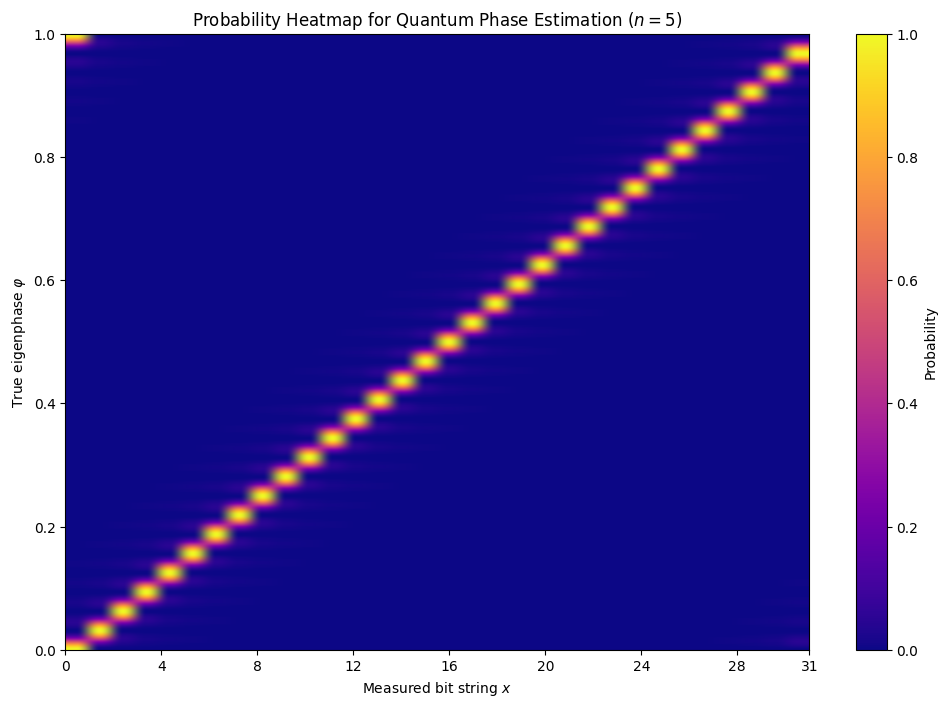
\includegraphics[scale=0.45]{qpe_heatmap.png}
    
\end{frame}

%%%%%%%%%%%%%%%%%%%%%%%%%%%%%%%%%%%%%%%%%%%%%%%%%%%%%%%%%%%%%%%%%%%%%%%%%%%

\begin{frame}{Physics Applications of Quantum Phase Estimation}

Quantum methods can efficiently simulate the time evolution:
\[
U_t = \exp(-i H t)
\]
for a large class of physical Hamiltonians (e.g., local Hamiltonians).

\bigskip
Applying QPE to $U_t$ enables:

\begin{itemize}
    \item Resolving the energies of $H$ (idealized).

    \medskip
    \item Implementing projectors onto low-energy states, which -- combined with amplitude amplification -- can prepare quantum states supported on low energies.

    \medskip
    \item Implementing jump operators $S(\omega)$ for Bohr frequencies $\omega$, facilitating the simulation of a Davies generator (Lindbladian) to prepare thermal states.
\end{itemize}

\smallskip
\textit{Note: Perfect energy resolution is not feasible in practice.}
\end{frame}


%%%%%%%%%%%%%%%%%%%%%%%%%%%%%%%%%%%%%%%%%%%%%%%%%%%%%%%%%%%%%%%%%%%%%%%%%%%

\begin{frame}{Shor's Algorithm: Quantum Phase Estimation Approach}

\textbf{Reduction:}

\medskip
Factoring

\quad \quad $\Downarrow$ 

Order finding

\quad \quad $\Downarrow$ 

Phase estimation of a unitary 

\end{frame}

%%%%%%%%%%%%%%%%%%%%%%%%%%%%%%%%%%%%%%%%%%%%%%%%%%%%%%%%%%%%%%%%%%%%%%%%%%%


\begin{frame}{Order Finding}

Given $a,N \in \Z$ with $\gcd(a,N)=1$, the \textbf{order} of $a$ modulo $N$ is the smallest positive integer $r$ such that $a^r \equiv 1 \pmod N$.

\bigskip

\begin{itemize}
\item Given: $a,N \in \Z$ with $\gcd(a,N)=1$

\medskip
\item Task: find the order $r$ of $a$ modulo $N$
\end{itemize}

\end{frame}

%%%%%%%%%%%%%%%%%%%%%%%%%%%%%%%%%%%%%%%%%%%%%%%%%%%%%%%%%%%%%%%%%%%%%%%%%%%

\begin{frame}{Reduction of Factoring to Order Finding}
  
Choose $a \in \{2,3,\ldots,N-1\}$ uniformly at random.

\bigskip

If $\gcd(a,N) \ne 1$, then it is a nontrivial factor of $N$.

\bigskip

If $\gcd(a,N)=1$, let $r$ denote the order of $a$ modulo $N$.

\bigskip
Output $\gcd(a^{r/2}-1,N)$ as a non-trivial factor of $N$.

\bigskip

\bigskip

This succeeds with large probability.

\end{frame}

%%

\begin{frame}{Example Reduction for Small $N$}

\bigskip
Consider $N=15$ and $a=7$:
\[
7^1=7,\quad 
7^2 \equiv 4,\quad 
7^3 \equiv 13,\quad 
7^4 \equiv 1 \quad \Longrightarrow\quad r=4
\]

We have
\[
\gcd(a^{r/2}-1,N) = \gcd(7^2-1,15)=\gcd(48, 15)=3
\]

\end{frame}

%%%%%%%%%%%%%%%%%%%%%%%%%%%%%%%%%%%%%%%%%%%%%%%%%%%%%%%%%%%%%%%%%%%%%%%%%%%%%%%%

\begin{frame}{Order Finding via Quantum Phase Estimation}

Order finding can be understood as applying quantum phase estimation to the unitary:
\[
U|x\> = |a x \pmod{N}\>,
\]
where $x \in \{0, 1, \ldots, N-1\}$.

\bigskip
When restricted to the invariant subspace $|1\>, |a\>, \ldots, |a^{r-1}\>$, $U$ is isomorphic to a cyclic shift modulo $r$.

\bigskip
The eigenphases of the cyclic shift operator are fractions:
\[
\frac{k}{r}, \quad k \in \{0, \ldots, r-1\}.
\]
The denominator $r$ is the order.

\bigskip
We obtain samples close to these fractions and recover the order $r$.
\end{frame}

%%%%%%%%%%%%%%%%%%%%%%%%%%%%%%%%%%%%%%%%%%%%%%%%%%%%%%%%%%%%%%%%%%%%%%%%%%%%%%%%

\begin{frame}{Shor's Algorithm as a Hidden Subgroup Problem over $\mathbb{Z}$}

Define the function:
\[
f: \mathbb{Z} \to \mathbb{Z}_N, \quad x \mapsto a^x \pmod{N}.
\]

This function is:

\medskip
\begin{itemize}
    \item Periodic with period $r$

    \medskip
    \item Injective within each period
\end{itemize}

\medskip
The symmetry is characterized by the \textbf{hidden subgroup} $H=r\Z$.
\end{frame}

%%%%%%%%%%%%%%%%%%%%%%%%%%%%%%%%%%%%%%%%%%%%%%%%%%%%%%%%%%%%%%%%%%%%%%%%%%%%%%%%

\begin{frame}{Function Evaluation in Input Superposition}

\begin{itemize}
    \item Since $\mathbb{Z}$ is infinite, we use a finite window $[0, \ldots, W-1]$ with $W=2^n$ on a quantum computer.

    \medskip
    \item Evaluate $f$ in superposition over the window:

    \medskip
    \[
    \frac{1}{\sqrt{W}} \sum_{x=0}^{W-1} |x\> \otimes |f(x)\>.
    \]

    \item This quantum state encodes the function graph of $f$.
\end{itemize}
\end{frame}

\begin{frame}{Example Function Graph}

    \bigskip
    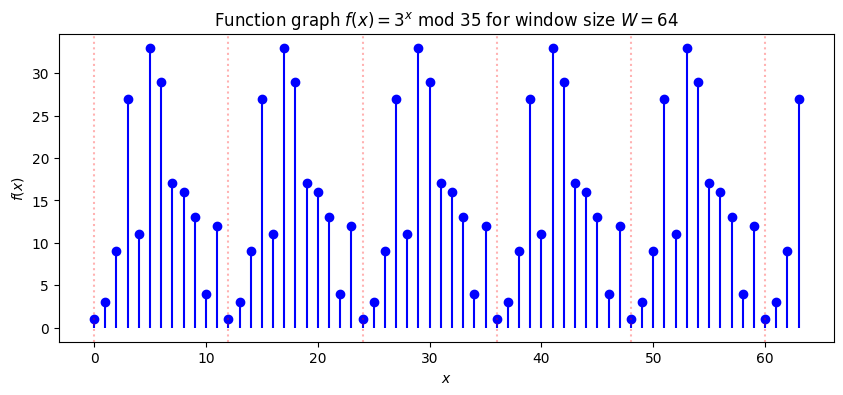
\includegraphics[scale=0.5]{modular_exponentiation.png}
\end{frame}

%%%%%%%%%%%%%%%%%%%%%%%%%%%%%%%%%%%%%%%%%%%%%%%%%%%%%%%%%%%%%%%%%%%%%%%%%%%%%%%%

\begin{frame}{Collapse onto Preimage After Output Measurement}

Let $y \in \mathrm{Im}(f)$. The preimage of $y$ is the set:
\[
f^{-1}(y) = \{ x \in \mathbb{Z}_W : f(x) = y \} = \{ b + \ell \cdot r \},
\]
where $b$ is the smallest value in the window with $f(b) = y$ and $\ell$ ranges over all values such that $b + \ell r < W$.

\bigskip
Measuring the output register collapses the input register into a \textbf{translated comb state} with offset $b$ and period $r$.
\end{frame}


%%%%%%%%%%%%%%%%%%%%%%%%%%%%%%%%%%%%%%%%%%%%%%%%%%%%%%%%%%%%%%%%%%%%%%%%%%%%%%%%

\begin{frame}{Perfect Periodicity, No Offset}
    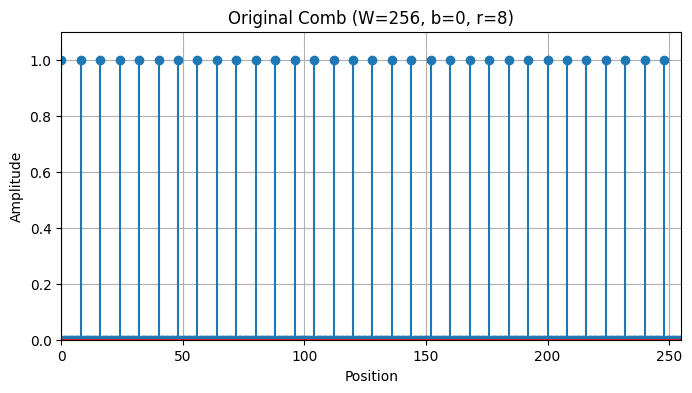
\includegraphics[scale=0.4]{comb_b0_r8.png}
    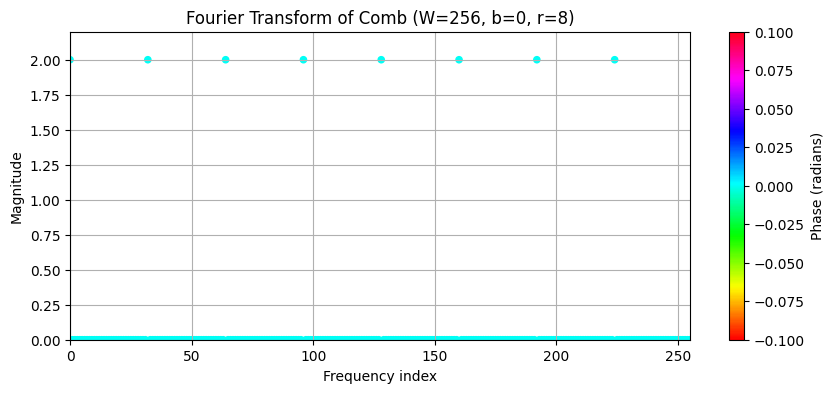
\includegraphics[scale=0.4]{fourier_comb_b0_r8.png}
\end{frame}

%%%%%%%%%%%%%%%%%%%%%%%%%%%%%%%%%%%%%%%%%%%%%%%%%%%%%%%%%%%%%%%%%%%%%%%%%%%%%%%%

\begin{frame}{Perfect Periodicity, Offset}
    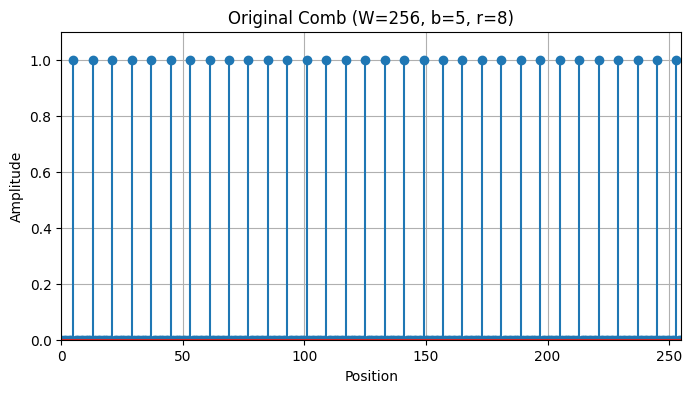
\includegraphics[scale=0.4]{comb_b5_r8.png}
    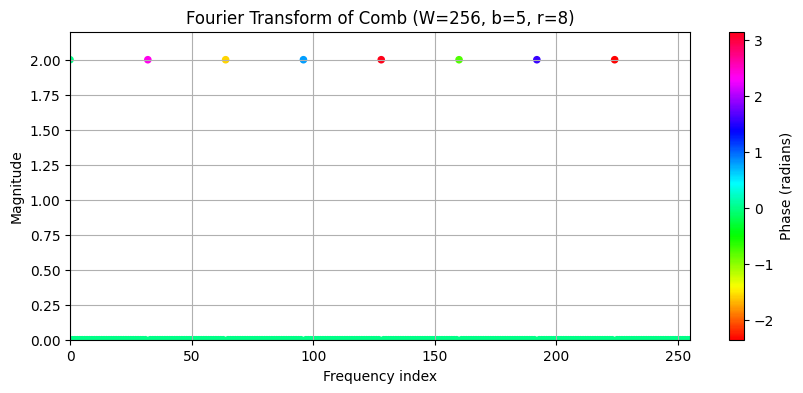
\includegraphics[scale=0.4]{fourier_comb_b5_r8.png}
\end{frame}

%%%%%%%%%%%%%%%%%%%%%%%%%%%%%%%%%%%%%%%%%%%%%%%%%%%%%%%%%%%%%%%%%%%%%%%%%%%%%%%%

\begin{frame}{Imperfect Periodicity}
    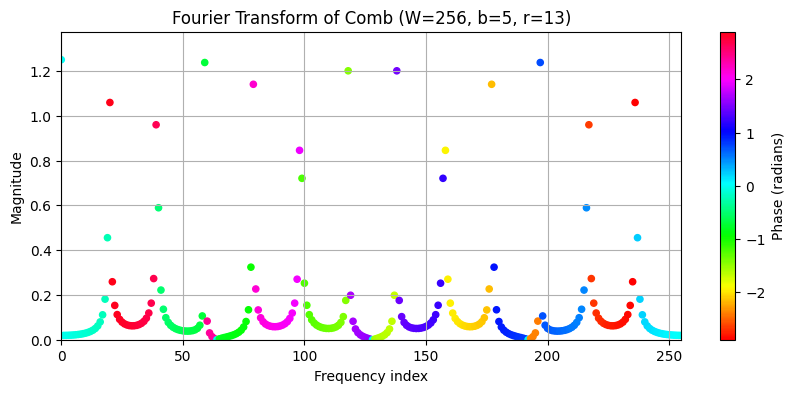
\includegraphics[scale=0.5]{fourier_comb_b5_r13.png}
\end{frame}

%%%%%%%%%%%%%%%%%%%%%%%%%%%%%%%%%%%%%%%%%%%%%%%%%%%%%%%%%%%%%%%%%%%%%%%%%%%%%%%%

\begin{frame}{Imperfect Periodicity, Larger Window}
    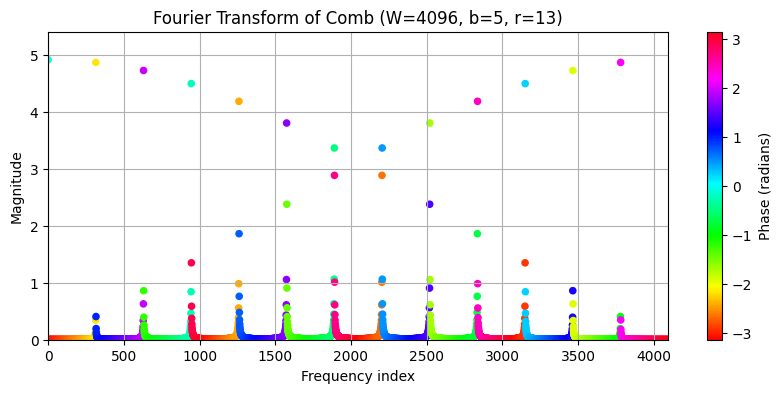
\includegraphics[scale=0.5]{fourier_comb_b5_r13_larger.png}
\end{frame}

%%%%%%%%%%%%%%%%%%%%%%%%%%%%%%%%%%%%%%%%%%%%%%%%%%%%%%%%%%%%%%%%%%%%%%%%%%%%%%%%

\begin{frame}{Hidden Subgroup Problem}
\begin{itemize}
    \item Let $G$ be a group and $H$ a subgroup.

    \medskip
    \item Let $f : G \rightarrow S$ (where $S$ is some set) be a function such that
    \begin{align*}
        f(g) = f(g') \quad \Longleftrightarrow \quad gH = g'H
    \end{align*}
    In words, two group elements $g$ and $g'$ have the same image under $f$ if and only if they are in the same coset in $G/H$.

    \medskip
    \item Task: given an oracle for $f$, determine the hidden subgroup $H$.
\end{itemize}
\end{frame}

%%%%%%%%%%%%%%%%%%%%%%%%%%%%%%%%%%%%%%%%%%%%%%%%%%%%%%%%%%%%%%%%%%%%%%%%%%%%%%%%

\begin{frame}{Hidden Subgroup Problem: Algorithms and Applications}
\begin{itemize}
    \item Efficient quantum algorithms exist for finite abelian and some finite non-abelian groups. 

    \bigskip
    \item Efficient quantum algorithms also exist for the infinite abelian groups $(\Z,+)$ and $(\R^n,+)$.

    \bigskip

    \bigskip
    \item Graph isomorphism can be cast the HSP over the symmetric group $S_n$.

    \bigskip
    \item Shor's algorithm for factoring solves the HSP over $\Z$.

    \bigskip
    \item Shor's algorithm for the DLOG problem in $\F_q^*$ solves the HSP over $\Z_N\times\Z_N$ for $N=q-1$.
\end{itemize}
\end{frame}

%%%%%%%%%%%%%%%%%%%%%%%%%%%%%%%%%%%%%%%%%%%%%%%%%%%%%%%%%%%%%%%%%%%%%%%%%%%%%%

\begin{frame}{Quantum Algorithm for Abelian HSP: Preparing a Random Coset State}

\begin{itemize}
\item We prepare the function graph state:
\begin{align*}
    \frac{1}{\sqrt{|G|}} \sum_{g \in G} |g\> \otimes |f(g)\> 
\end{align*}

\bigskip
\item Measuring the output register collapses the input register onto a random coset state:
\begin{align*}
|t + H\> 
&= 
\frac{1}{\sqrt{|H|}} \sum_{h \in H} |t + h\>,
\end{align*}

where $ t \in T $ and $ T $ is a transversal for the coset space $ G/H $.
\end{itemize}
\end{frame}

%%%%%%%%%%%%%%%%%%%%%%%%%%%%%%%%%%%%%%%%%%%%%%%%%%%%%%%%%%%%%%%%%%%%%%%%%%%%%%%%

\begin{frame}{QAlgo for Abelian HSP: Pontragyagin Duality}
    
    \begin{itemize}
        \item Pontragyagin duality establishes an isomorphism $\varphi$ between a finite abelian group $G$ and its character group $\hat{G} = \mathrm{Hom}(G, \mathbb{C}^\times)$.
        
        \medskip
        \item This isomorphism allows us to \textbf{identify} $G$ with $\hat{G}$, mapping each element $g \in G$ to a character $\chi_g \in \hat{G}$.
        
        \medskip
        \item For a subgroup $H \leq G$, the dual subgroup $H^\perp$ is defined as:
        \[
            H^\perp = \{ g \in G : \chi_g(h) = 1 \quad \forall h \in H \}.
        \]

        In words, $H^\perp$ is the collection of characters than annihilate each element in $H$.
    
    \end{itemize}
\end{frame}

%%%%%%%%%%%%%%%%%%%%%%%%%%%%%%%%%%%%%%%%%%%%%%%%%%%%%%%%%%%%%%%%%%%%%%%%%%%%%%


\begin{frame}{QAlgo for Abelian HSP: Fourier Transform and Recovery}
    \begin{itemize}
        \item The quantum Fourier transform $F_G$ over $G$ is given by:
        \[
            F_G = \frac{1}{\sqrt{|G|}} \sum_{g,g' \in G} \chi_g(g') |g'\>\<g|
        \]
    
        \item It maps the uniform superposition over $H$ to the uniform superposition over $H^\perp$:
        \[
            F_G |H\> = |H^\perp\>
        \]
    
        \item Using an oracle for $f$, we prepare a random coset state:
        \[
            |t + H\>
        \]
        
        \item Applying $F_G$ to $|t+H\>$ yields a phase-modulated $|H^\perp\>$.

        \medskip
        \item We can sample uniformly at random from $H^\perp$ and recover the hidden subgroup $H$.
    \end{itemize}
\end{frame}

%%%%%%%%%%%%%%%%%%%%%%%%%%%%%%%%%%%%%%%%%%%%%%%%%%%%%%%%%%%%%%%%%%%%%%%%%%%%%%

\begin{frame}{Non-Abelian Fourier Transforms: A Bird’s-Eye View}

\begin{itemize}
    \item The \textbf{quantum Fourier transform for a group $G$} decomposes \textbf{coset states} into components corresponding to the \textbf{irreducible representations} of $G$.
    %
    \begin{center}
        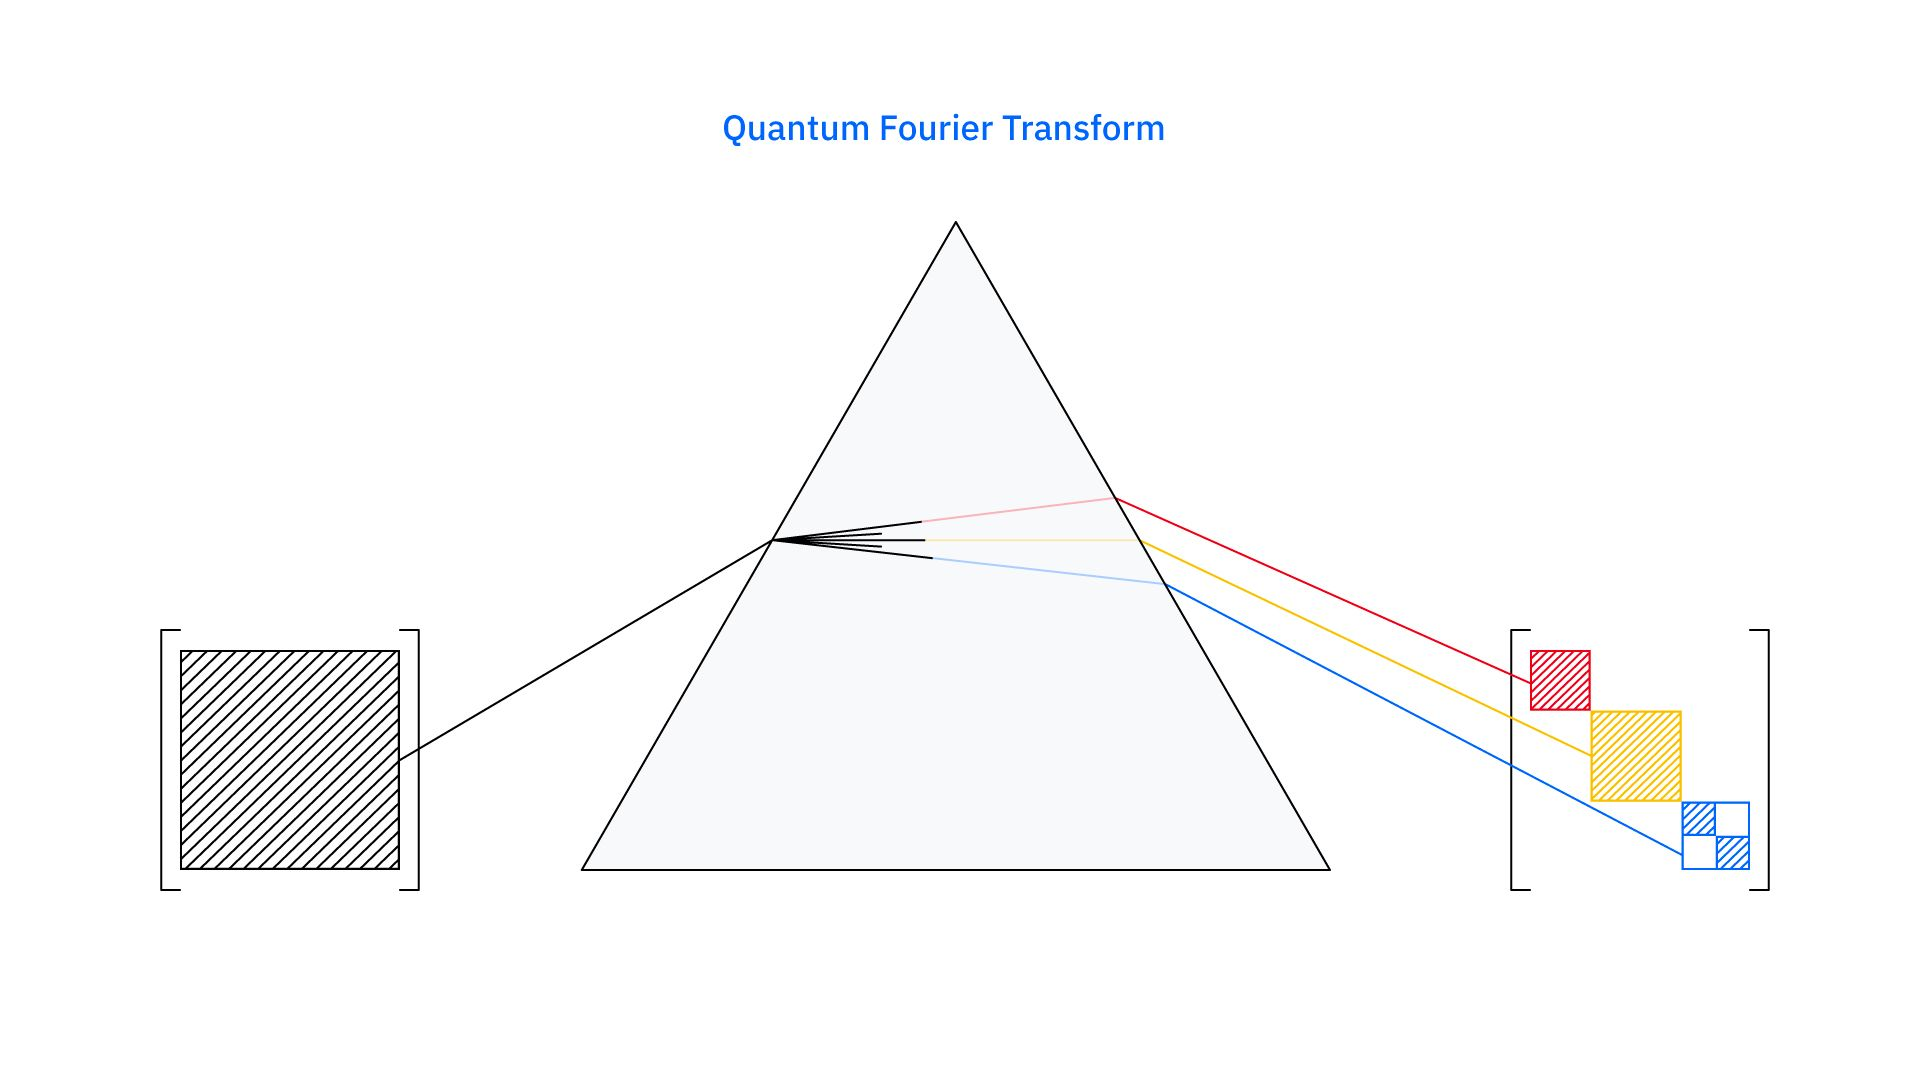
\includegraphics[width=0.9\textwidth]{non-abelian-QFT.jpg}
    \end{center}
    %
    \item For \textbf{Abelian groups}, these representations are one-dimensional.

\end{itemize}
\end{frame}

%%%%%%%%%%%%%%%%%%%%%%%%%%%%%%%%%%%%%%%%%%%%%%%%%%%%%%%%%%%%%%%%%%%%%%%%%%%%%%


\begin{frame}{Non-Abelian Fourier Transforms: Recent Progress by IBM}

\begin{itemize}
    \item While QFT has been successful for \textbf{Abelian groups} , its extension to \textbf{non-Abelian groups} has historically faced challenges.

    \medskip
    
    \item Recent work by IBM researchers has demonstrated a \textbf{quantum algorithm for non-Abelian Fourier transforms}, specifically for the symmetric group.

    \medskip
    \url{https://www.ibm.com/quantum/blog/group-theory}
    
    \medskip

    \item This algorithm provides a \textbf{potential quantum speedup} for computing Kronecker coefficients and other multiplicities, with implications for algebraic combinatorics and quantum advantage.
\end{itemize}
\end{frame}


\begin{frame}{Resources for Quantum Algorithms}

\begin{itemize}
    \item \textbf{Book:}
    \textit{An Introduction to Quantum Computing} by Phillip Kaye, Raymond Laflamme, and Michele Mosca

    \medskip
    \item \textbf{Lecture Notes:}
    \textit{Lecture Notes on Quantum Algorithms} by Andrew Childs: \url{https://www.cs.umd.edu/~amchilds/qa/}
    
    \medskip
    \item \textbf{Recent Developments:}
    For more recent topics such as 

    \medskip
    \begin{itemize}
        \item \textit{block encoding \& quantum signal transform} 
        
        \medskip
        \item \textit{decoded quantum interferometry}
        
        \medskip
        \item \textit{quantum Gibbs sampling} 
    \end{itemize}

    \medskip
    it is best to consult original research articles, arXiv preprints, or tutorials on platforms like YouTube.
\end{itemize}
\end{frame}


\end{document}